% ================================================
% KHUNG LATEX CHO REPORT DATABASE SYSTEM OF DORM
% Dựa trên phân tích REPORT.pdf
% ================================================

\documentclass[12pt,a4paper]{report}

% ================================
% PHẦN 1: KHAI BÁO CÁC GÓI (PACKAGES)
% ================================

% Gói hỗ trợ tiếng Việt (nếu cần)
% \usepackage[utf8]{vietnam}
% \usepackage[utf8]{inputenc}


% Gói cho font và mã hóa
\usepackage[T1]{fontenc}
\usepackage{lmodern}

% Gói cho đồ họa và hình ảnh
\usepackage{graphicx}
\usepackage{float}

% Gói cho bảng
\usepackage{array}
\usepackage{tabularx}
\usepackage{multirow}
\usepackage{booktabs}
%
\usepackage[utf8]{inputenc}
\usepackage{graphicx} % BẮT BUỘC: Gói này dùng để chèn ảnh
\usepackage{lipsum}   % Gói này chỉ để tạo văn bản giả, em có thể xóa đi
% Gói cho code SQL
\usepackage{listings}
\usepackage{xcolor}

% Thiết lập cho code listings
\lstset{
    basicstyle=\ttfamily\small,
    keywordstyle=\color{blue}\bfseries,
    commentstyle=\color{green!60!black},
    stringstyle=\color{red},
    showstringspaces=false,
    breaklines=true,
    frame=single,
    numbers=left,
    numberstyle=\tiny\color{gray},
    language=SQL
}

% Gói cho liên kết
\usepackage{hyperref}
\hypersetup{
    colorlinks=true,
    linkcolor=blue,
    filecolor=magenta,      
    urlcolor=cyan,
    pdftitle={Database System Report},
    pdfauthor={Student Name},
}

% Gói cho margins
\usepackage{geometry}
\geometry{
    a4paper,
    left=2cm,
    right=1cm,
    top=3cm,
    bottom=2cm
}

% Gói cho header và footer
\usepackage{fancyhdr}
\pagestyle{fancy}
\fancyhf{}
\fancyhead[L]{\leftmark}
\fancyhead[R]{\thepage}
\renewcommand{\headrulewidth}{0.4pt}
% ================================
% ================================
% PHẦN MACRO CHO LAYOUT TEXT + IMAGE (CĂNG CHỈNH NGANG)
% ================================

\newcommand{\textimage}[3]{%
  \noindent
  \begin{minipage}[c]{0.48\textwidth}
    \raggedright
    #1
  \end{minipage}
  \hfill
  \begin{minipage}[c]{0.48\textwidth}
    \centering
    \includegraphics[width=\textwidth]{#2}
    
    \small{\textit{#3}}
  \end{minipage}
  
  \vspace{1.5cm}
}



% ================================
% PHẦN 2: THÔNG TIN TRANG BÌA
% ================================

\title{
    \textbf{DATABASE SYSTEM}\\
    \textbf{MANAGE LEARNING GOALS OF STUDENTS}\\
    \textbf{FPT UNIVERSITY}\\
    \vspace{2cm}
    \LARGE ASSIGNMENT
}

\author{
    \textbf{GROUP: 04}\\[0.5cm]
    \makebox[\textwidth][3]{
        \begin{tabular}{l}
        STUDENT NAME: VU HONG QUAN | HE19xxxx\\
        STUDENT NAME: NGUYEN VIET HOANG  | HE19xxxx\\
        STUDENT NAME: PHAN CONG MINH THANH  | HE19xxxx
        \end{tabular}
    }\\[1cm]
    INSTRUCTOR: Dr. PHAN NGOC HOANG, Ph.D
}


\date{November 07, 2025}





% ================================
% PHẦN 3: BẮT ĐẦU TÀI LIỆU
% ================================

\begin{document}

% Trang bìa
\maketitle
\newpage

% Mục lục
\tableofcontents
\newpage

% ================================
% CHAPTER I: INTRODUCE THE PROBLEM
% ================================

\chapter{INTRODUCE THE PROBLEM}

\section{DESCRIBE THE PROBLEM}

Nowadays, Students at FPT University set academic and personal goals to track their performance and skill development. However, there is no centralized database system to manage these objectives, track their progress, or link them to academic advisors. After analyzing the provided database schema (\verb|FPTU_LearningGoalManagement|), the business rules are as follows:

\begin{itemize}
    \item A student can define multiple learning goals. Each goal belongs to exactly one student. (1-N relationship from \verb|Student| to \verb|LearningGoal|).
    \item Each student can be assigned an \verb|Instructor| as an academic advisor. This relationship is tracked over time, and a student can have only one active advisor at a time.
    \item The system records information about students, including: \verb|StudentID| (e.g., 'SE160001'), \verb|FirstName|, \verb|LastName|, \verb|Email|, \verb|Major|, and \verb|GPA|. The \verb|GPA| must be between 0.00 and 4.00.
    \item A learning goal has a \verb|GoalTitle|, \verb|TargetValue| (e.g., 'GPA: 3.8'), \verb|StartDate|, and \verb|Deadline|. The \verb|Deadline| must be later than the \verb|StartDate|.
    \item Each goal is categorized (e.g., 'Academic', 'Skill Development') and has a status ('Active', 'Completed', 'Failed', 'Cancelled'), managed by lookup tables.
    \item Progress for a goal (\verb|ProgressTracking|) can be updated by the student who owns the goal or by their currently assigned active advisor. Data consistency and security are ensured by triggers.
    \item A goal can have multiple \verb|Milestone| (sub-tasks). The \verb|DueDate| of a milestone cannot be after the \verb|Deadline| of its parent goal.
    \item The system also manages student \verb|Enrollment| in courses, recording the \verb|Instructor|, \verb|MidtermScore|, and \verb|FinalScore| for each course in a specific \verb|Semester|.
\end{itemize}

\section{MANAGEMENT OBJECTIVES}

\begin{itemize}
    \item Manage student information and academic enrollments.
    \item Manage student-defined learning goals, milestones, and progress history.
    \item Manage the assignment of instructors as academic advisors.
    \item Manage course information, scores, and academic semesters.
    \item Enforce data consistency and security automatically through triggers.
\end{itemize}

\textbf{Important output:}
\begin{itemize}
    \item A summary report of all student goals with their latest progress and time status.
    \item A calculated academic transcript showing average scores and grades.
    \item A report of all currently active student-advisor pairings.
    \item A detailed report of milestone status (Pending, Completed, Overdue) for each goal.
\end{itemize}

% ================================
% CHƯƠNG II: ENTITY-RELATIONSHIP
% ================================

\chapter{ENTITY -- RELATIONSHIP -- ERD}

\section{DEFINITION ENTITY -- ATTRIBUTE}

Based on the problem description and management objectives from Chapter I, we can present several entities and attributes of the entity as follows

\begin{itemize}
    \item \textbf{GoalCategoryLookup}: CategoryID (PK), CategoryName, Description, IsActive
    \item \textbf{GoalStatusLookup}: StatusID (PK), StatusName, Description, IsActive
    \item \textbf{SemesterLookup}: SemesterID (PK), SemesterCode, StartDate, EndDate, IsActive
    \item \textbf{Instructor}: InstructorID (PK), FirstName, LastName, Email, Department, Phone, HireDate, IsActive
    \item \textbf{Student}: StudentID (PK), FirstName, LastName, Email, Major, GPA, EnrollmentDate, Phone, IsActive
    \item \textbf{Course}: CourseID (PK), CourseName, Credits, Description, IsActive
    \item \textbf{Enrollment}: EnrollmentID (PK), StudentID (FK), CourseID (FK), SemesterID (FK), InstructorID (FK), MidtermScore, FinalScore, EnrollmentDate
    \item \textbf{LearningGoal}: GoalID (PK), StudentID (FK), CategoryID (FK), GoalTitle, GoalDescription, TargetValue, StartDate, Deadline, StatusID (FK), CreatedDate, LastModifiedDate
    \item \textbf{ProgressTracking}: TrackingID (PK), GoalID (FK), ProgressPercent, Notes, TrackingDate, UpdatedBy
    \item \textbf{Milestone}: MilestoneID (PK), GoalID (FK), MilestoneName, Description, DueDate, CompletedDate, CreatedDate
    \item \textbf{AdvisorAssignment}: AssignmentID (PK), StudentID (FK), InstructorID (FK), AssignedDate, UnassignedDate
\end{itemize}

\section{SET-UP ENTITY -- RELATIONSHIP}

\subsection*{Some symbols used in the model}

%============================
\textimage{
  \begin{itemize}
    \item Key / identifier attribute
    \vspace{1cm}
    \item Attribute description / description
    \vspace{1cm}
    \item Entity
\vspace{1cm}
    \item Weak entity
    \vspace{1cm}
    \item Relationship
     \vspace{1cm}
    \item Connectivity (force) = 1
    \vspace{1cm}
    \item Connectivity = N
    \vspace{1cm}
  \end{itemize}
}{symbols.png}{Entity Relationship Diagram Symbols}


% Chèn ER Diagram ở đây
 \begin{figure}[H]
    \centering
    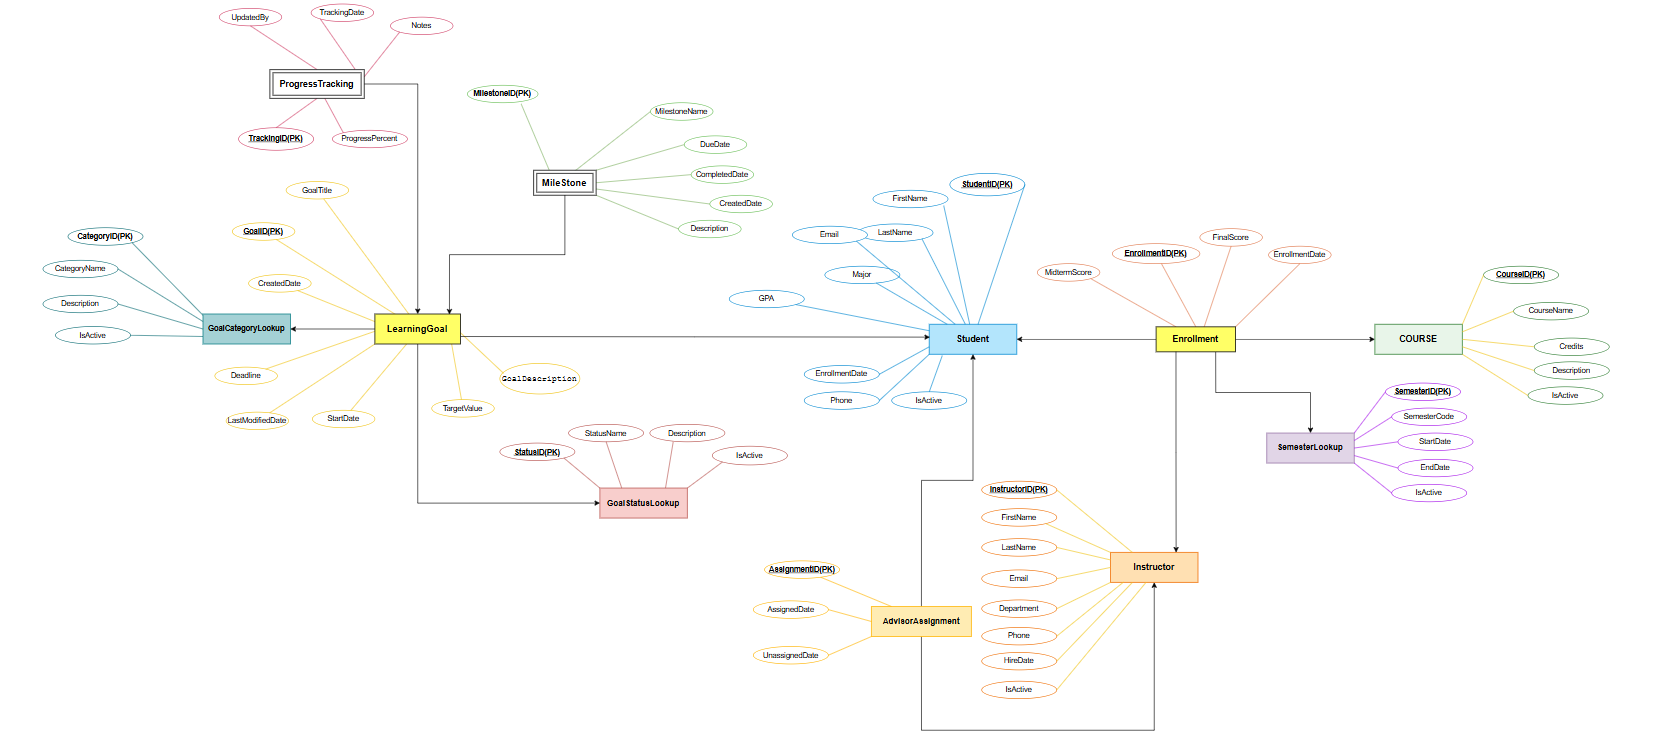
\includegraphics[width=\textwidth]{ERD.png}
    \caption{Entity Relationship Diagram}
\end{figure}

% ================================
% CHƯƠNG III: DATA DICTIONARY
% ================================

\chapter{DATA DICTIONARY}

\section{DATABASE AND TABLE}

\subsection{CREATE DATABASE }

\begin{lstlisting}[language=SQL, caption=Create Database (\texttt{FPTU\_LearningGoalManagement})]
-- Create database FPTU_LearningGoalManagement
CREATE DATABASE FPTU_LearningGoalManagement;
\end{lstlisting}

 \begin{figure}[H]
    \centering
    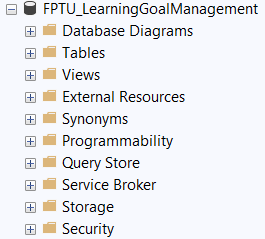
\includegraphics[width=0.2\textwidth]{create_table.png}
    \caption{Entity Relationship Diagram}
 \end{figure}



\subsection{CREATE TABLE GoalCategoryLookup}

\textbf{Column Definition:GoalCategoryLookup}


%=============
\begin{table}[h!]
\centering
\renewcommand{\arraystretch}{1.2} % Tăng chiều cao của hàng một chút cho dễ đọc
\begin{tabular}{|l|l|l|l|l|}
\hline
\textbf{Column Name} & \textbf{Data Type} & \textbf{Default} & \textbf{Check} & \textbf{Key/ Index/ Constraint} \\ \hline
CategoryID     & INT            &                  &                & PRIMARY KEY, IDENTITY(1,1)    \\ \hline
CategoryName   & NVARCHAR(50)   &                  &                & NOT NULL, UNIQUE              \\ \hline
Description    & NVARCHAR(200)  &                  &                &                               \\ \hline
IsActive       & BIT            & 1                &                &                               \\ \hline
\end{tabular}
\caption{Table Schema for GoalCategoryLookup}
\label{tab:goal_category_lookup}
\end{table}


%=============
\vspace{1cm}
\vspace{1cm}
\vspace{1cm}

\begin{lstlisting}[language=SQL, caption=Create Table GoalCategoryLookup]
-- Create table guard
    CREATE TABLE GoalCategoryLookup (
    CategoryID INT PRIMARY KEY IDENTITY(1,1),
    CategoryName NVARCHAR(50) NOT NULL UNIQUE,
    Description NVARCHAR(200),
    IsActive BIT DEFAULT 1
);

\end{lstlisting}
\textbf{Example Data}
\begin{table}[h!]
\centering
% Cột 'p{6cm}' cho phép cột 'Description' tự động xuống dòng.
\begin{tabular}{|l|l|p{8cm}|l|}
\hline
\textbf{CategoryID} & \textbf{CategoryName} & \textbf{Description} & \textbf{IsActive} \\ \hline
1 & Academic & Goals related to study, GPA, and grades & 1 \\ \hline
2 & Skill Development & Professional and technical skill development & 1 \\ \hline
3 & Career & Career goals, internships, and employment & 1 \\ \hline
4 & Personal & Personal goals, health, and self-improvement & 1 \\ \hline
5 & Project & Project completion and assignment goals & 1 \\ \hline
6 & Certificate & Professional certification goals & 1 \\ \hline
\end{tabular}
\caption{Data for GoalCategoryLookup}
\label{tab:goal_category_data}
\end{table}




% TABLE 2: GoalStatusLookup
% ========================================================================================
\subsection{CREATE TABLE GoalStatusLookup}

\textbf{Column Definition: GoalStatusLookup}

\begin{table}[ht]
\centering
\small
\begin{tabular}{|l|l|l|l|l|}
\hline
\textbf{Column Name} & \textbf{Data Type} & \textbf{Default} & \textbf{Check} & \textbf{Key/Constraint} \\ \hline
StatusID & INT & & & PK, IDENTITY(1,1) \\ \hline
StatusName & NVARCHAR(30) & & IN values & NOT NULL, UNIQUE \\ \hline
Description & NVARCHAR(200) & & & \\ \hline
IsActive & BIT & 1 & & \\ \hline
\end{tabular}
\caption{Table Schema for GoalStatusLookup}
\label{tab:goal_status_lookup_schema}
\end{table}

\vspace{0.3cm}

\begin{lstlisting}[language=SQL, caption=Create Table GoalStatusLookup]
CREATE TABLE GoalStatusLookup (
    StatusID INT PRIMARY KEY IDENTITY(1,1),
    StatusName NVARCHAR(30) NOT NULL UNIQUE 
        CHECK(StatusName IN ('Active', 'Completed', 
                             'Failed', 'Cancelled')),
    Description NVARCHAR(200),
    IsActive BIT DEFAULT 1
);
\end{lstlisting}
\vspace{1cm}
\textbf{Example Data}

\begin{table}[ht]
\centering
\small
\begin{tabular}{|c|l|p{4.5cm}|c|}
\hline
\textbf{StatusID} & \textbf{StatusName} & \textbf{Description} & \textbf{IsActive} \\ \hline
1 & Active & Goal is currently in progress & 1 \\ \hline
2 & Completed & Goal has been successfully completed & 1 \\ \hline
3 & Failed & Goal has failed & 1 \\ \hline
4 & Cancelled & Goal has been cancelled & 1 \\ \hline
\end{tabular}
\caption{Sample Data for GoalStatusLookup}
\label{tab:goal_status_lookup_data}
\end{table}

\vspace{1cm}

% TABLE 3: SemesterLookup
% ========================================================================================
\subsection{CREATE TABLE SemesterLookup}

\textbf{Column Definition: SemesterLookup}

\begin{table}[ht]
\centering
\small
\begin{tabular}{|l|l|l|l|l|}
\hline
\textbf{Column Name} & \textbf{Data Type} & \textbf{Default} & \textbf{Check} & \textbf{Key/Constraint} \\ \hline
SemesterID & INT & & & PK, IDENTITY(1,1) \\ \hline
SemesterCode & VARCHAR(20) & & & NOT NULL, UNIQUE \\ \hline
StartDate & DATE & & & NOT NULL \\ \hline
EndDate & DATE & & EndDate $>$ Start & NOT NULL \\ \hline
IsActive & BIT & 1 & & \\ \hline
\end{tabular}
\caption{Table Schema for SemesterLookup}
\label{tab:semester_lookup_schema}
\end{table}

\vspace{0.3cm}

\begin{lstlisting}[language=SQL, caption=Create Table SemesterLookup]
CREATE TABLE SemesterLookup (
    SemesterID INT PRIMARY KEY IDENTITY(1,1),
    SemesterCode VARCHAR(20) NOT NULL UNIQUE,
    StartDate DATE NOT NULL,
    EndDate DATE NOT NULL,
    IsActive BIT DEFAULT 1,
    CHECK(EndDate > StartDate)
);
\end{lstlisting}

\textbf{Example Data}

\begin{table}[ht]
\centering
\small
\begin{tabular}{|c|l|l|l|c|}
\hline
\textbf{SemesterID} & \textbf{SemesterCode} & \textbf{StartDate} & \textbf{EndDate} & \textbf{IsActive} \\ \hline
1 & Fall2024 & 2024-09-01 & 2024-12-31 & 1 \\ \hline
2 & Spring2025 & 2025-01-01 & 2025-05-31 & 1 \\ \hline
3 & Summer2025 & 2025-06-01 & 2025-08-31 & 1 \\ \hline
4 & Fall2025 & 2025-09-01 & 2025-12-31 & 1 \\ \hline
\end{tabular}
\caption{Sample Data for SemesterLookup}
\label{tab:semester_lookup_data}
\end{table}

\vspace{1cm}

% 
% TABLE 4: Instructor
% ========================================================================================
\subsection{CREATE TABLE Instructor}

\textbf{Column Definition: Instructor}

\begin{table}[ht]
\centering
\small
\begin{tabular}{|l|l|l|l|l|}
\hline
\textbf{Column Name} & \textbf{Data Type} & \textbf{Default} & \textbf{Check} & \textbf{Key/Constraint} \\ \hline
InstructorID & VARCHAR(10) & & LIKE pattern & PK \\ \hline
FirstName & NVARCHAR(50) & & & NOT NULL \\ \hline
LastName & NVARCHAR(50) & & & NOT NULL \\ \hline
Email & NVARCHAR(100) & & Email valid & UNIQUE, NOT NULL \\ \hline
Department & NVARCHAR(100) & & & NOT NULL \\ \hline
Phone & VARCHAR(15) & & & \\ \hline
HireDate & DATE & GETDATE() & & \\ \hline
IsActive & BIT & 1 & & \\ \hline
\end{tabular}
\caption{Table Schema for Instructor}
\label{tab:instructor_schema}
\end{table}

\vspace{0.3cm}

\begin{lstlisting}[language=SQL, caption=Create Table Instructor]
CREATE TABLE Instructor (
    InstructorID VARCHAR(10) PRIMARY KEY 
        CHECK(InstructorID LIKE 'INS[0-9][0-9][0-9][0-9][0-9]'),
    FirstName NVARCHAR(50) NOT NULL,
    LastName NVARCHAR(50) NOT NULL,
    Email NVARCHAR(100) NOT NULL UNIQUE 
        CHECK(Email LIKE '%_@__%.__%'),
    Department NVARCHAR(100) NOT NULL,
    Phone VARCHAR(15),
    HireDate DATE DEFAULT GETDATE(),
    IsActive BIT DEFAULT 1
);
\end{lstlisting}

\textbf{Example Data}

\begin{table}[ht]
\centering
\small
\begin{tabular}{|l|l|l|p{5cm}|p{4cm}|}
\hline
\textbf{InstructorID} & \textbf{FirstName} & \textbf{LastName} & \textbf{Email} & \textbf{Department} \\ \hline
INS00001 & John & Smith & john.smith@fptu.edu.vn & Software Engineering \\ \hline
INS00002 & Mary & Johnson & mary.johnson@fptu.edu.vn & Information Systems \\ \hline
INS00003 & David & Williams & david.williams@fptu.edu.vn & Artificial Intelligence \\ \hline
INS00004 & Sarah & Brown & sarah.brown@fptu.edu.vn & Software Engineering \\ \hline
INS00005 & Robert & Davis & robert.davis@fptu.edu.vn & Data Science \\ \hline
\end{tabular}
\caption{Sample Data for Instructor}
\label{tab:instructor_data}
\end{table}

\vspace{9cm}

% ========================================================================================
% TABLE 5: Student
% ========================================================================================
\subsection{CREATE TABLE Student}

\textbf{Column Definition: Student}

\begin{table}[ht]
\centering
\small
\begin{tabular}{|l|l|l|l|l|}
\hline
\textbf{Column Name} & \textbf{Data Type} & \textbf{Default} & \textbf{Check} & \textbf{Key/Constraint} \\ \hline
StudentID & VARCHAR(10) & & LIKE pattern & PK \\ \hline
FirstName & NVARCHAR(50) & & & NOT NULL \\ \hline
LastName & NVARCHAR(50) & & & NOT NULL \\ \hline
Email & NVARCHAR(100) & & Email valid & UNIQUE, NOT NULL \\ \hline
Major & NVARCHAR(100) & & & NOT NULL \\ \hline
GPA & DECIMAL(3,2) & 0.00 & 0.00--4.00 & \\ \hline
EnrollmentDate & DATE & GETDATE() & & \\ \hline
Phone & VARCHAR(15) & & & \\ \hline
IsActive & BIT & 1 & & \\ \hline
\end{tabular}
\caption{Table Schema for Student}
\label{tab:student_schema}
\end{table}

\vspace{0.3cm}

\begin{lstlisting}[language=SQL, caption=Create Table Student]
CREATE TABLE Student (
    StudentID VARCHAR(10) PRIMARY KEY 
        CHECK(
            (StudentID LIKE 'SE[0-9][0-9][0-9][0-9][0-9][0-9]') 
            OR (StudentID LIKE 'HE[0-9][0-9][0-9][0-9][0-9][0-9]') 
            OR (StudentID LIKE 'SS[0-9][0-9][0-9][0-9][0-9][0-9]')
        ),
    FirstName NVARCHAR(50) NOT NULL,
    LastName NVARCHAR(50) NOT NULL,
    Email NVARCHAR(100) NOT NULL UNIQUE 
        CHECK(Email LIKE '%_@__%.__%'),
    Major NVARCHAR(100) NOT NULL,
    GPA DECIMAL(3,2) DEFAULT 0.00 
        CHECK(GPA >= 0.00 AND GPA <= 4.00),
    EnrollmentDate DATE DEFAULT GETDATE(),
    Phone VARCHAR(15),
    IsActive BIT DEFAULT 1
);
\end{lstlisting}

\textbf{Example Data}

\begin{table}[ht]
\centering
\small
\begin{tabular}{|l|l|l|p{4.2cm}|p{4.2cm}|c|}
\hline
\textbf{StudentID} & \textbf{FirstName} & \textbf{LastName} & \textbf{Email} & \textbf{Major} & \textbf{GPA} \\ \hline
SE160001 & Nguyen & Van A & anvse160001@fpt.edu.vn & Software Engineering & 3.50 \\ \hline
SE160002 & Tran & Thi B & bttse160002@fpt.edu.vn & Software Engineering & 3.75 \\ \hline
HE160001 & Pham & Thi D & dtphe160001@fpt.edu.vn & Information Systems & 3.60 \\ \hline
HE160002 & Hoang & Minh E & emhe160002@fpt.edu.vn & Information Systems & 3.40 \\ \hline
SS160001 & Vu & Thanh F & ftvss160001@fpt.edu.vn & Software Engineering & 3.80 \\ \hline
\end{tabular}
\caption{Sample Data for Student}
\label{tab:student_data}
\end{table}

\vspace{1cm}

% ========================================================================================
% TABLE 6: Course
% ========================================================================================
\subsection{CREATE TABLE Course}

\textbf{Column Definition: Course}

\begin{table}[ht]
\centering
\small
\begin{tabular}{|l|l|l|l|l|}
\hline
\textbf{Column Name} & \textbf{Data Type} & \textbf{Default} & \textbf{Check} & \textbf{Key/Constraint} \\ \hline
CourseID & VARCHAR(10) & & LIKE pattern & PK \\ \hline
CourseName & NVARCHAR(200) & & & NOT NULL \\ \hline
Credits & INT & & 1--6 & NOT NULL \\ \hline
Description & NVARCHAR(500) & & & \\ \hline
IsActive & BIT & 1 & & \\ \hline
\end{tabular}
\caption{Table Schema for Course}
\label{tab:course_schema}
\end{table}

\vspace{0.3cm}

\begin{lstlisting}[language=SQL, caption=Create Table Course]
CREATE TABLE Course (
    CourseID VARCHAR(10) PRIMARY KEY 
        CHECK(CourseID LIKE '[A-Z][A-Z][A-Z][0-9][0-9][0-9]'),
    CourseName NVARCHAR(200) NOT NULL,
    Credits INT NOT NULL CHECK(Credits > 0 AND Credits <= 6),
    Description NVARCHAR(500),
    IsActive BIT DEFAULT 1
);
\end{lstlisting}

\textbf{Example Data}

\begin{table}[ht]
\centering
\small
\begin{tabular}{|l|l|c|p{5cm}|}
\hline
\textbf{CourseID} & \textbf{CourseName} & \textbf{Credits} & \textbf{Description} \\ \hline
DBI202 & Introduction to Databases & 3 & Database design, SQL, normalization \\ \hline
PRJ301 & Java Web Application & 3 & Web application development \\ \hline
SWE201 & Software Engineering & 3 & SDLC, Agile, processes \\ \hline
MAE101 & Math for Engineers & 4 & Advanced math, linear algebra \\ \hline
AID101 & AI Basics & 3 & Introduction to AI and ML \\ \hline
\end{tabular}
\caption{Sample Data for Course}
\label{tab:course_data}
\end{table}

\vspace{8cm}

% ========================================================================================
% TABLE 7: Enrollment
% ========================================================================================
\subsection{CREATE TABLE Enrollment}

\textbf{Column Definition: Enrollment}

\begin{table}[ht]
\centering
\small
\begin{tabular}{|l|l|l|l|l|}
\hline
\textbf{Column Name} & \textbf{Data Type} & \textbf{Default} & \textbf{Check} & \textbf{Key/Constraint} \\ \hline
EnrollmentID & INT & & & PK, IDENTITY(1,1) \\ \hline
StudentID & VARCHAR(10) & & & FK, NOT NULL \\ \hline
CourseID & VARCHAR(10) & & & FK, NOT NULL \\ \hline
SemesterID & INT & & & FK, NOT NULL \\ \hline
InstructorID & VARCHAR(10) & NULL & & FK \\ \hline
MidtermScore & DECIMAL(5,2) & & 0--10 & \\ \hline
FinalScore & DECIMAL(5,2) & & 0--10 & \\ \hline
EnrollmentDate & DATE & GETDATE() & & \\ \hline
\end{tabular}
\caption{Table Schema for Enrollment}
\label{tab:enrollment_schema}
\end{table}

\vspace{0.3cm}

\begin{lstlisting}[language=SQL, caption=Create Table Enrollment]
CREATE TABLE Enrollment (
    EnrollmentID INT PRIMARY KEY IDENTITY(1,1),
    StudentID VARCHAR(10) NOT NULL,
    CourseID VARCHAR(10) NOT NULL,
    SemesterID INT NOT NULL,
    InstructorID VARCHAR(10) NULL,
    MidtermScore DECIMAL(5,2) 
        CHECK(MidtermScore >= 0 AND MidtermScore <= 10),
    FinalScore DECIMAL(5,2) 
        CHECK(FinalScore >= 0 AND FinalScore <= 10),
    EnrollmentDate DATE DEFAULT GETDATE(),
    UNIQUE(StudentID, CourseID, SemesterID),
    FOREIGN KEY (StudentID) REFERENCES Student(StudentID) 
        ON DELETE NO ACTION ON UPDATE CASCADE,
    FOREIGN KEY (CourseID) REFERENCES Course(CourseID) 
        ON DELETE NO ACTION ON UPDATE CASCADE,
    FOREIGN KEY (SemesterID) REFERENCES SemesterLookup(SemesterID)
        ON DELETE NO ACTION,
    FOREIGN KEY (InstructorID) REFERENCES Instructor(InstructorID)
        ON DELETE SET NULL
);
\end{lstlisting}

\textbf{Example Data}

\begin{table}[ht]
\centering
\small
\begin{tabular}{|c|l|l|c|l|c|c|}
\hline
\textbf{EnrollID} & \textbf{StudentID} & \textbf{CourseID} & \textbf{SemID} & \textbf{InstructorID} & \textbf{Midterm} & \textbf{Final} \\ \hline
1 & SE160001 & DBI202 & 1 & INS00001 & 8.5 & 9.0 \\ \hline
2 & SE160001 & PRJ301 & 1 & INS00002 & 7.5 & 8.0 \\ \hline
3 & SE160002 & DBI202 & 1 & INS00001 & 9.0 & 9.5 \\ \hline
9 & SE160001 & WEB301 & 2 & INS00002 & NULL & NULL \\ \hline
10 & SE160002 & MLE401 & 2 & INS00005 & 8.8 & 9.2 \\ \hline
\end{tabular}
\caption{Sample Data for Enrollment}
\label{tab:enrollment_data}
\end{table}

\vspace{1cm}

% ========================================================================================
% TABLE 8: LearningGoal
% ========================================================================================
\subsection{CREATE TABLE LearningGoal}

\textbf{Column Definition: LearningGoal}

\begin{table}[ht]
\centering
\small
\begin{tabular}{|l|l|l|l|l|}
\hline
\textbf{Column Name} & \textbf{Data Type} & \textbf{Default} & \textbf{Check} & \textbf{Key/Constraint} \\ \hline
GoalID & INT & & & PK, IDENTITY(1,1) \\ \hline
StudentID & VARCHAR(10) & & & FK, NOT NULL \\ \hline
CategoryID & INT & & & FK, NOT NULL \\ \hline
GoalTitle & NVARCHAR(200) & & & NOT NULL \\ \hline
GoalDescription & NVARCHAR(500) & & & \\ \hline
TargetValue & NVARCHAR(100) & & & NOT NULL \\ \hline
StartDate & DATE & GETDATE() & & NOT NULL \\ \hline
Deadline & DATE & & Deadline $>$ Start & NOT NULL \\ \hline
StatusID & INT & 1 & & FK, NOT NULL \\ \hline
CreatedDate & DATETIME & GETDATE() & & \\ \hline
LastModifiedDate & DATETIME & GETDATE() & & \\ \hline
\end{tabular}
\caption{Table Schema for LearningGoal}
\label{tab:learning_goal_schema}
\end{table}



\begin{lstlisting}[language=SQL, caption=Create Table LearningGoal]
CREATE TABLE LearningGoal (
    GoalID INT PRIMARY KEY IDENTITY(1,1),
    StudentID VARCHAR(10) NOT NULL,
    CategoryID INT NOT NULL, 
    GoalTitle NVARCHAR(200) NOT NULL,
    GoalDescription NVARCHAR(500),
    TargetValue NVARCHAR(100) NOT NULL,
    StartDate DATE NOT NULL DEFAULT GETDATE(),
    Deadline DATE NOT NULL,
    StatusID INT NOT NULL DEFAULT 1,
    CreatedDate DATETIME DEFAULT GETDATE(),
    LastModifiedDate DATETIME DEFAULT GETDATE(),
    FOREIGN KEY (StudentID) REFERENCES Student(StudentID) 
        ON DELETE NO ACTION ON UPDATE CASCADE,
    FOREIGN KEY (CategoryID) 
        REFERENCES GoalCategoryLookup(CategoryID),
    FOREIGN KEY (StatusID) 
        REFERENCES GoalStatusLookup(StatusID),
    CHECK(Deadline > StartDate)
);
\end{lstlisting}
\vspace{0.5cm}
\textbf{Example Data}
\begin{table}[ht]
\centering
\small
\begin{tabular}{|c|l|c|p{4cm}|l|l|}
\hline
\textbf{GoalID} & \textbf{StudentID} & \textbf{Cat} & \textbf{GoalTitle} & \textbf{TargetValue} & \textbf{Deadline} \\ \hline
1 & SE160001 & 1 & Achieve GPA 3.8 & GPA: 3.8 & 2024-12-31 \\ \hline
2 & SE160001 & 2 & AWS Certification & Certificate & 2025-03-31 \\ \hline
3 & SE160001 & 3 & FPT Internship & Job Offer & 2025-02-28 \\ \hline
4 & SE160002 & 1 & Maintain GPA 3.7 & GPA: 3.7+ & 2024-12-31 \\ \hline
5 & SE160002 & 5 & Capstone Project & Grade: A & 2025-05-31 \\ \hline
\end{tabular}
\caption{Sample Data for LearningGoal}
\label{tab:learning_goal_data}
\end{table}
\vspace{3cm}
% ========================================================================================
% TABLE 9: ProgressTracking
% ========================================================================================
\subsection{CREATE TABLE ProgressTracking}

\textbf{Column Definition: ProgressTracking}

\textit{Design Decision (Security):} UpdatedBy is VARCHAR (not FK) to allow both StudentID and InstructorID.

\begin{table}[ht]
\centering
\small
\begin{tabular}{|l|l|l|l|l|}
\hline
\textbf{Column Name} & \textbf{Data Type} & \textbf{Default} & \textbf{Check} & \textbf{Key/Constraint} \\ \hline
TrackingID & INT & & & PK, IDENTITY(1,1) \\ \hline
GoalID & INT & & & FK, NOT NULL \\ \hline
ProgressPercent & DECIMAL(5,2) & & 0--100 & NOT NULL \\ \hline
Notes & NVARCHAR(500) & & & \\ \hline
TrackingDate & DATETIME & GETDATE() & & NOT NULL \\ \hline
UpdatedBy & VARCHAR(10) & & & NOT NULL \\ \hline
\end{tabular}
\caption{Table Schema for ProgressTracking}
\label{tab:progress_tracking_schema}
\end{table}

\begin{lstlisting}[language=SQL, caption=Create Table ProgressTracking]
CREATE TABLE ProgressTracking (
    TrackingID INT PRIMARY KEY IDENTITY(1,1),
    GoalID INT NOT NULL,
    ProgressPercent DECIMAL(5,2) NOT NULL 
        CHECK(ProgressPercent >= 0 AND ProgressPercent <= 100),
    Notes NVARCHAR(500),
    TrackingDate DATETIME NOT NULL DEFAULT GETDATE(),
    UpdatedBy VARCHAR(10) NOT NULL,
    FOREIGN KEY (GoalID) REFERENCES LearningGoal(GoalID) 
        ON DELETE CASCADE ON UPDATE CASCADE
);
\end{lstlisting}

\textbf{Example Data}

\begin{table}[ht]
\centering
\small
\begin{tabular}{|c|c|c|p{8cm}|l|}
\hline
\textbf{TrackingID} & \textbf{GoalID} & \textbf{Progress\%} & \textbf{Notes} & \textbf{UpdatedBy} \\ \hline
1 & 1 & 25.00 & Completed 2 of 8 courses, average 3.5 & SE160001 \\ \hline
2 & 1 & 50.00 & Midterm results good, current GPA 3.6 & SE160001 \\ \hline
3 & 1 & 75.00 & Continued progress, 5 of 8 courses completed & INS00001 \\ \hline
4 & 1 & 100.00 & Completed. Final GPA 3.82 & SE160001 \\ \hline
5 & 2 & 20.00 & Completed module 1 on Udemy & SE160001 \\ \hline
\end{tabular}
\caption{Sample Data for ProgressTracking}
\label{tab:progress_tracking_data}
\end{table}

\vspace{5cm}

% 
% TABLE 10: Milestone
% ========================================================================================
\subsection{CREATE TABLE Milestone}

\textbf{Column Definition: Milestone}
\begin{table}[ht]
\centering
\small
\begin{tabular}{|l|l|l|l|l|}
\hline
\textbf{Column Name} & \textbf{Data Type} & \textbf{Default} & \textbf{Check} & \textbf{Key/Constraint} \\ \hline
MilestoneID & INT & & & PK, IDENTITY(1,1) \\ \hline
GoalID & INT & & & FK, NOT NULL \\ \hline
MilestoneName & NVARCHAR(200) & & & NOT NULL \\ \hline
Description & NVARCHAR(500) & & & \\ \hline
DueDate & DATE & & & NOT NULL \\ \hline
CompletedDate & DATE & & Comp $\geq$ Created & \\ \hline
CreatedDate & DATETIME & & & NOT NULL \\ \hline
\end{tabular}
\caption{Table Schema for Milestone}
\label{tab:milestone_schema}
\end{table}

\vspace{0.3cm}

\begin{lstlisting}[language=SQL, caption=Create Table Milestone]
CREATE TABLE Milestone (
    MilestoneID INT PRIMARY KEY IDENTITY(1,1),
    GoalID INT NOT NULL,
    MilestoneName NVARCHAR(200) NOT NULL,
    Description NVARCHAR(500),
    DueDate DATE NOT NULL,
    CompletedDate DATE,
    CreatedDate DATETIME NOT NULL,
    CHECK(CompletedDate IS NULL 
          OR CompletedDate >= CreatedDate),
    FOREIGN KEY (GoalID) REFERENCES LearningGoal(GoalID) 
        ON DELETE CASCADE ON UPDATE CASCADE
);
\end{lstlisting}

\textbf{Example Data}

\begin{table}[ht]
\centering
\small
\begin{tabular}{|c|c|p{5cm}|l|l|l|}
\hline
\textbf{MilestoneID} & \textbf{GoalID} & \textbf{MilestoneName} & \textbf{DueDate} & \textbf{CompletedDate} & \textbf{CreatedDate} \\ \hline
1 & 1 & Midterm Exams & 2024-10-31 & 2024-10-30 & 2024-09-01 \\ \hline
2 & 1 & Final Exams & 2024-12-20 & 2024-12-25 & 2024-09-01 \\ \hline
3 & 1 & Final GPA Check & 2024-12-31 & 2024-12-26 & 2024-09-01 \\ \hline
4 & 2 & Complete AWS Course & 2024-12-31 & NULL & 2024-09-01 \\ \hline
10 & 5 & Design Document & 2024-10-30 & 2024-10-28 & 2024-09-01 \\ \hline
\end{tabular}
\caption{Sample Data for Milestone}
\label{tab:milestone_data}
\end{table}

\vspace{5cm}

% ========================================================================================
% TABLE 11: AdvisorAssignment
% ========================================================================================
\subsection{CREATE TABLE AdvisorAssignment}

\textbf{Column Definition: AdvisorAssignment}

\begin{table}[ht]
\centering
\small
\begin{tabular}{|l|l|l|l|l|}
\hline
\textbf{Column Name} & \textbf{Data Type} & \textbf{Default} & \textbf{Check} & \textbf{Key/Constraint} \\ \hline
AssignmentID & INT & & & PK, IDENTITY(1,1) \\ \hline
StudentID & VARCHAR(10) & & & FK, NOT NULL \\ \hline
InstructorID & VARCHAR(10) & & & FK, NOT NULL \\ \hline
AssignedDate & DATE & GETDATE() & & NOT NULL \\ \hline
UnassignedDate & DATE & & Unassign $>$ Assign & \\ \hline
\end{tabular}
\caption{Table Schema for AdvisorAssignment}
\label{tab:advisor_assignment_schema}
\end{table}

\begin{lstlisting}[language=SQL, caption=Create Table AdvisorAssignment]
CREATE TABLE AdvisorAssignment (
    AssignmentID INT PRIMARY KEY IDENTITY(1,1),
    StudentID VARCHAR(10) NOT NULL,
    InstructorID VARCHAR(10) NOT NULL,
    AssignedDate DATE NOT NULL DEFAULT GETDATE(),
    UnassignedDate DATE,
    FOREIGN KEY (StudentID) REFERENCES Student(StudentID) 
        ON DELETE NO ACTION ON UPDATE CASCADE,
    FOREIGN KEY (InstructorID) REFERENCES Instructor(InstructorID) 
        ON DELETE NO ACTION ON UPDATE CASCADE,
    CHECK(UnassignedDate IS NULL 
          OR UnassignedDate > AssignedDate)
);
\end{lstlisting}

\textbf{Example Data}

\begin{table}[ht]
\centering
\small
\begin{tabular}{|c|l|l|l|l|l|}
\hline
\textbf{AssignmentID} & \textbf{StudentID} & \textbf{InstructorID} & \textbf{AssignedDate} & \textbf{UnassignedDate} & \textbf{Status} \\ \hline
1 & SE160001 & INS00001 & 2024-09-01 & NULL & Active \\ \hline
2 & SE160002 & INS00001 & 2024-09-01 & NULL & Active \\ \hline
3 & HE160001 & INS00002 & 2024-09-01 & 2025-01-31 & Inactive \\ \hline
4 & HE160002 & INS00003 & 2024-09-01 & NULL & Active \\ \hline
5 & SS160001 & INS00004 & 2024-09-01 & NULL & Active \\ \hline
\end{tabular}
\caption{Sample Data for AdvisorAssignment}
\label{tab:advisor_assignment_data}
\end{table}

\vspace{6cm}

% ========================================================================================
% TABLE 12: AuditLog
% ========================================================================================
\subsection{CREATE TABLE AuditLog}

\textbf{Column Definition: AuditLog}

\begin{table}[ht]
\centering
\small
\begin{tabular}{|l|l|l|l|l|}
\hline
\textbf{Column Name} & \textbf{Data Type} & \textbf{Default} & \textbf{Check} & \textbf{Key/Constraint} \\ \hline
LogID & INT & & & PK, IDENTITY(1,1) \\ \hline
TableName & NVARCHAR(50) & & & NOT NULL \\ \hline
Operation & NVARCHAR(20) & & IN (I,U,D) & NOT NULL \\ \hline
RecordID & NVARCHAR(100) & & & NOT NULL \\ \hline
OldValue & NVARCHAR(MAX) & & & \\ \hline
NewValue & NVARCHAR(MAX) & & & \\ \hline
ModifiedBy & VARCHAR(10) & & & \\ \hline
ModifiedDate & DATETIME & GETDATE() & & \\ \hline
\end{tabular}
\caption{Table Schema for AuditLog}
\label{tab:audit_log_schema}
\end{table}

\vspace{0.3cm}

\begin{lstlisting}[language=SQL, caption=Create Table AuditLog]
CREATE TABLE AuditLog (
    LogID INT PRIMARY KEY IDENTITY(1,1),
    TableName NVARCHAR(50) NOT NULL,
    Operation NVARCHAR(20) NOT NULL 
        CHECK(Operation IN ('INSERT', 'UPDATE', 'DELETE')),
    RecordID NVARCHAR(100) NOT NULL,
    OldValue NVARCHAR(MAX),
    NewValue NVARCHAR(MAX),
    ModifiedBy VARCHAR(10),
    ModifiedDate DATETIME DEFAULT GETDATE()
);
\end{lstlisting}

\textbf{Example Data}

\begin{table}[ht]
\centering
\small
\begin{tabular}{|c|l|l|l|l|}
\hline
\textbf{LogID} & \textbf{TableName} & \textbf{Operation} & \textbf{RecordID} & \textbf{ModifiedBy} \\ \hline
1 & LearningGoal & INSERT & 1 & SE160001 \\ \hline
2 & LearningGoal & UPDATE & 1 & SE160001 \\ \hline
3 & ProgressTracking & INSERT & 4 & SE160001 \\ \hline
4 & Enrollment & INSERT & 1 & SYSTEM \\ \hline
5 & AdvisorAssignment & UPDATE & 4 & HE160001 \\ \hline
\end{tabular}
\caption{Sample Data for AuditLog}
\label{tab:audit_log_data}
\end{table}


% ================================
% CHƯƠNG IV: ERD
% ================================

\chapter{ENTITY RELATIONSHIP DIAGRAM (ERD)}

\section{STUDENT}
 \begin{figure}[H]
     \centering
    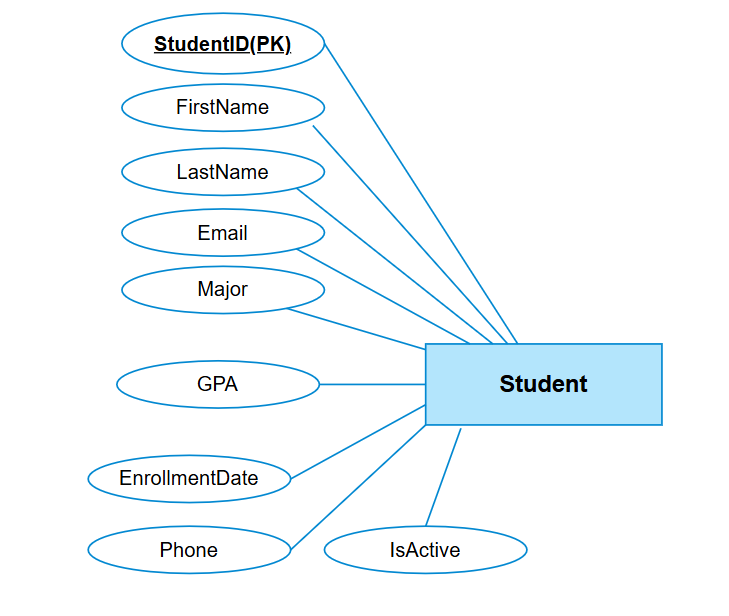
\includegraphics[width=0.6\textwidth]{student.png}
    \caption{Student Entity}
\end{figure}
%================
\noindent
\begin{tabular}{p{0.55\textwidth}p{0.40\textwidth}}
\vspace{0pt}
This is the Student entity, representing students enrolled in the university. The Student entity has 9 attributes: StudentID (PK - Primary Key), FirstName, LastName, Email, Major, GPA, EnrollmentDate, Phone, and IsActive.
&
\vspace{0pt}
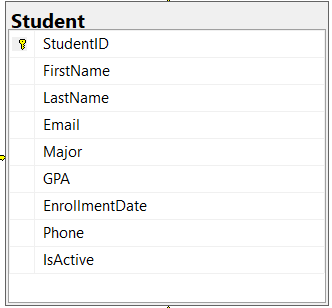
\includegraphics[width=0.95\linewidth]{student_tb.png}
\\
\end{tabular}

\vspace{1.5cm}

% SECTION 2: INSTRUCTOR ENTITY
% ========================================================================================



\section{INSTRUCTOR Entity}
\begin{figure}[H]
     \centering
    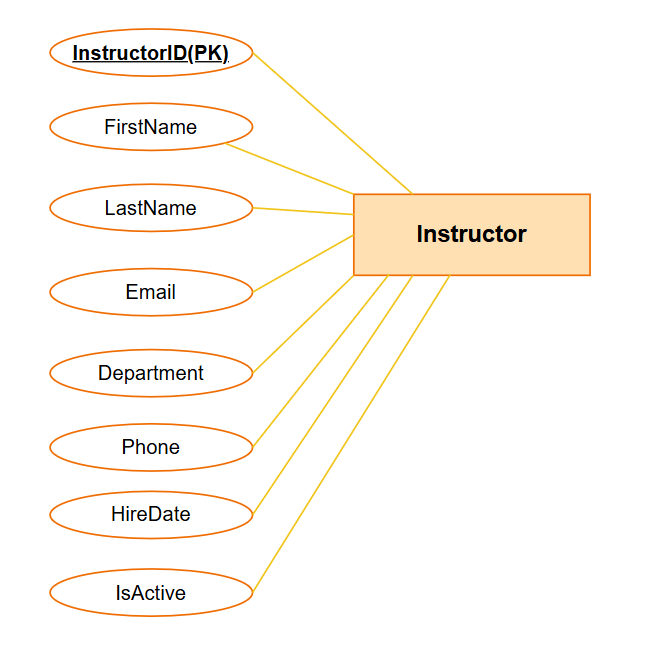
\includegraphics[width=0.6\textwidth]{instructor.png}
    \caption{}
\end{figure}
\noindent
\begin{tabular}{p{0.55\textwidth}p{0.40\textwidth}}
\vspace{0pt}
This is the Instructor entity, the secondary root of the diagram---faculty members who teach courses and advise students. Instructor has 8 attributes. InstructorID uniquely identifies each instructor using the format INS[0-9]{5} (e.g., INS00001, INS00042). Each instructor has Name information split into FirstName and LastName, enabling professional communication. Contact information comprises Email (UNIQUE, format ``[firstname].[lastname]@fptu.edu.vn'') and Phone. The Department attribute identifies the instructor's organizational unit (Software Engineering, Information Systems, Artificial Intelligence, Data Science). HireDate records employment start date, tracking tenure. IsActive indicates current employment status (1=Active, 0=Retired/On-leave). Only active instructors can teach courses and serve as student advisors.
&
\vspace{0pt}
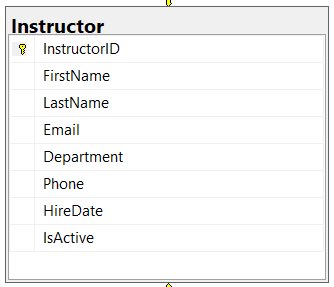
\includegraphics[width=0.95\linewidth]{instructor_tb.png}
\\
\end{tabular}

\vspace{1.5cm}

% ========================================================================================
% SECTION 3: COURSE ENTITY
% ========================================================================================

\section{COURSE Entity}
\begin{figure}[H]
     \centering
    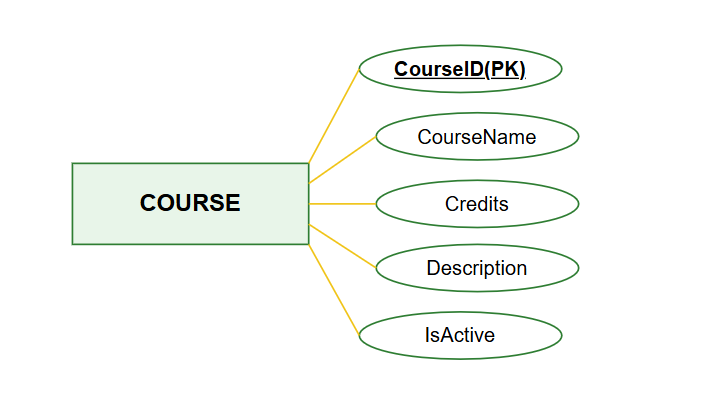
\includegraphics[width=0.8\textwidth]{course.png}
    \caption{}
\end{figure}
\noindent
\begin{tabular}{p{0.55\textwidth}p{0.40\textwidth}}
\vspace{0pt}
This is the Course entity, a static reference entity representing the course catalog. Course has 5 attributes. CourseID is the primary key using the format [A-Z][A-Z][A-Z][0-9][0-9][0-9] (e.g., DBI202, PRJ301, SWE201). CourseName is the full name of the course (e.g., ``Introduction to Databases''). Credits represents the academic credit hours, ranging from 1 to 6. Description provides detailed course objectives and content. IsActive indicates whether the course is currently offered (1) or discontinued (0). One course can have many enrollments across different semesters and instructors. This entity is independent and does not depend on other entities.
&
\vspace{0pt}
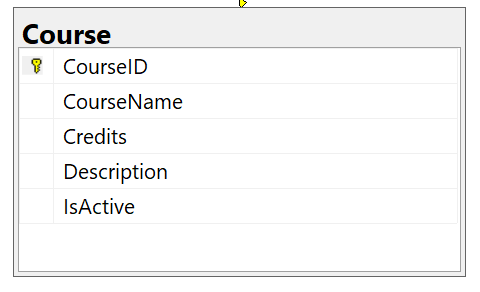
\includegraphics[width=0.95\linewidth]{course_tb.png}
\\
\end{tabular}

\vspace{1.5cm}

% SECTION 4: ENROLLMENT ENTITY
% ========================================================================================

\section{ENROLLMENT Entity}
\begin{figure}[H]
     \centering
    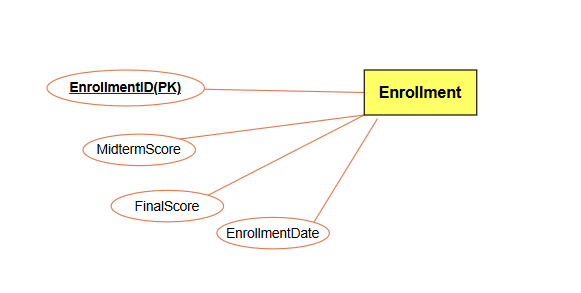
\includegraphics[width=0.8\textwidth]{errollment.png}
    \caption{}
\end{figure}
\noindent
\begin{tabular}{p{0.55\textwidth}p{0.40\textwidth}}
\vspace{0pt}
This is the Enrollment entity, a junction table representing the many-to-many relationship between Student and Course. Enrollment has 8 attributes. EnrollmentID is the auto-incremented primary key. StudentID (FK) references the Student entity. CourseID (FK) references the Course entity. SemesterID (FK) identifies which semester the enrollment occurs. InstructorID (FK, nullable) identifies the instructor teaching this course section. MidtermScore and FinalScore store exam results (0-10 range), with NULL values allowed for pending scores. EnrollmentDate records the registration date. A UNIQUE constraint ensures one student cannot enroll in the same course twice per semester. This entity connects students to their coursework and enables grade tracking.
&
\vspace{0pt}
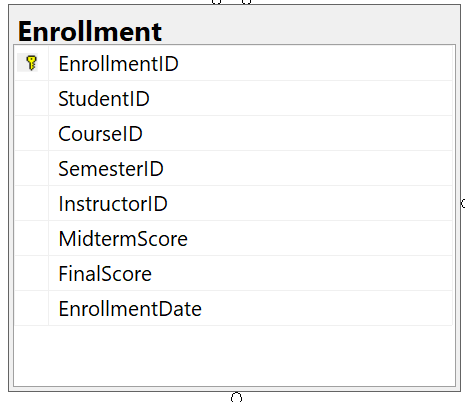
\includegraphics[width=0.95\linewidth]{errollment_tb.png}
\\
\end{tabular}

\vspace{1.5cm}

% ========================================================================================
% SECTION 5: LEARNINGGOAL ENTITY
% ========================================================================================

\section{LEARNINGGOAL Entity}
\begin{figure}[H]
     \centering
    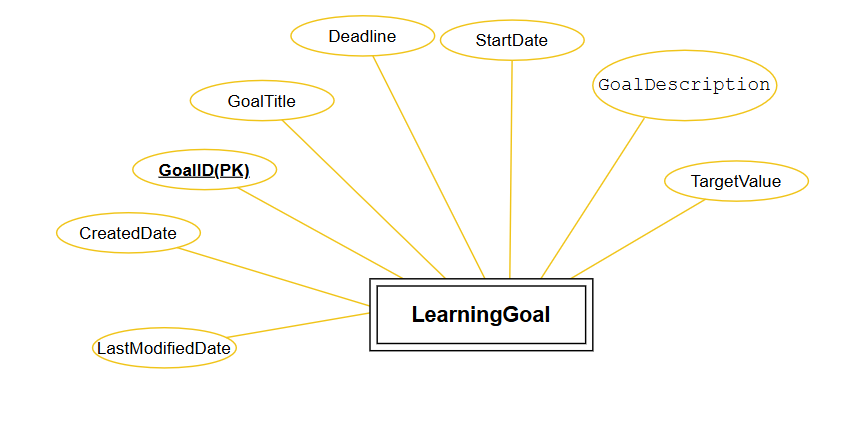
\includegraphics[width=0.8\textwidth]{learninggoal.png}
    \caption{}
\end{figure}
\noindent
\begin{tabular}{p{0.55\textwidth}p{0.40\textwidth}}
\vspace{0pt}
This is the LearningGoal entity, representing student-defined objectives within the goal management system. LearningGoal has 11 attributes. GoalID is the auto-incremented primary key. StudentID (FK) references the student who owns the goal. CategoryID (FK) links to GoalCategoryLookup (Academic, Skill, Career, Personal, Project, Certificate). GoalTitle and GoalDescription define the goal. TargetValue specifies the measurable target (e.g., ``GPA: 3.8'', ``Certificate Completion''). StartDate (default: TODAY) and Deadline define the goal timeframe. StatusID (FK) references GoalStatusLookup (Active, Completed, Failed, Cancelled). CreatedDate and LastModifiedDate track lifecycle. Each learning goal can have multiple progress tracking records and milestones, enabling detailed progress monitoring and goal decomposition.
&
\vspace{0pt}
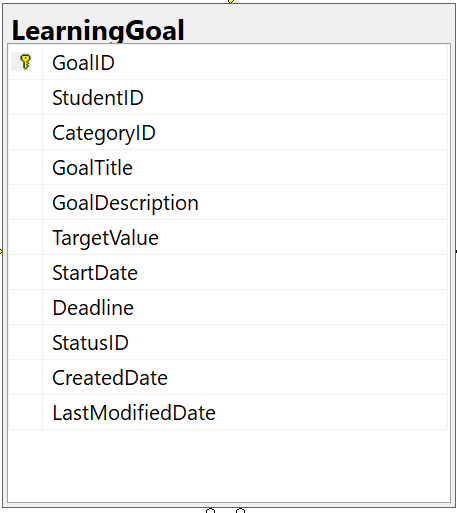
\includegraphics[width=0.95\linewidth]{learninggoal_tb.png}
\\
\end{tabular}

\vspace{1.5cm}

% ========================================================================================
% SECTION 6: PROGRESSTRACKING ENTITY
% ========================================================================================

\section{PROGRESSTRACKING Entity}
\begin{figure}[H]
     \centering
    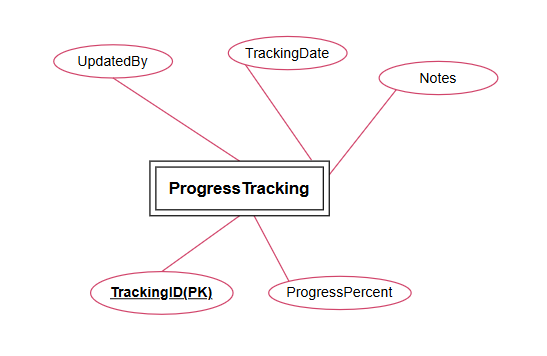
\includegraphics[width=0.8\textwidth]{progresstracking.png}
    \caption{}
\end{figure}
\noindent
\begin{tabular}{p{0.55\textwidth}p{0.40\textwidth}}
\vspace{0pt}
This is the ProgressTracking entity, which maintains a historical audit trail of all progress updates for learning goals. ProgressTracking has 6 attributes. TrackingID is the auto-incremented primary key. GoalID (FK) references the parent LearningGoal entity. ProgressPercent stores the progress percentage (0-100) with decimal precision. Notes field allows textual descriptions of progress (e.g., ``Completed module 1 on Udemy''). TrackingDate records when the update occurred (default: NOW). UpdatedBy is a VARCHAR field storing either StudentID or InstructorID (no FK to support both types). A CHECK constraint ensures ProgressPercent remains between 0 and 100. This entity uses ON DELETE CASCADE, meaning when a goal is deleted, all tracking records are automatically removed. Students and instructors can update progress collaboratively.
&
\vspace{0pt}
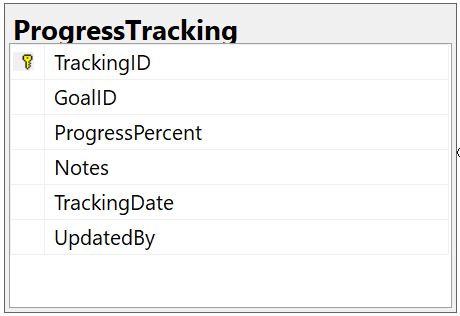
\includegraphics[width=0.95\linewidth]{progresstracking_tb.png}
\\
\end{tabular}

\vspace{1.5cm}

% ========================================================================================
% SECTION 7: MILESTONE ENTITY
% ========================================================================================

\section{MILESTONE Entity}
\begin{figure}[H]
     \centering
    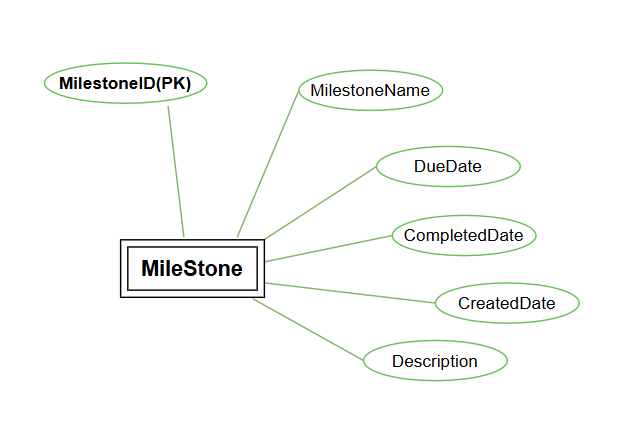
\includegraphics[width=0.8\textwidth]{milestone.png}
    \caption{}
\end{figure}
\noindent
\begin{tabular}{p{0.55\textwidth}p{0.40\textwidth}}
\vspace{0pt}
This is the Milestone entity, representing sub-goals or checkpoints within a learning goal (weak entity). Milestone has 7 attributes. MilestoneID is the auto-incremented primary key. GoalID (FK) references the parent LearningGoal and is required (weak entity identity). MilestoneName provides the milestone name. Description explains the milestone. DueDate sets the target completion date. CompletedDate records actual completion (NULL if incomplete). CreatedDate records creation timestamp and is NOT NULL to support historical data insertion. A CHECK constraint ensures CompletedDate is NULL or $\geq$ CreatedDate. This entity uses ON DELETE CASCADE, so deleting a goal removes all milestones. Milestones enable goal decomposition into manageable sub-tasks with individual tracking.
&
\vspace{0pt}
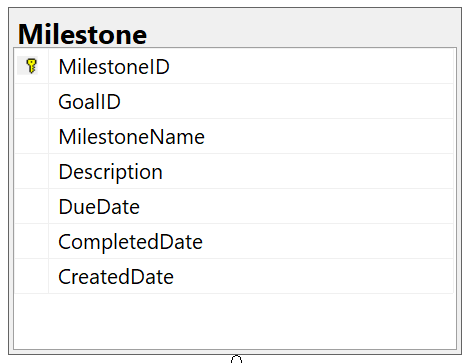
\includegraphics[width=0.95\linewidth]{milestone_tb.png}
\\
\end{tabular}

\vspace{1.5cm}

% ========================================================================================
% SECTION 8: ADVISORASSIGNMENT ENTITY
% ========================================================================================

\section{ADVISORASSIGNMENT Entity}
\begin{figure}[H]
     \centering
    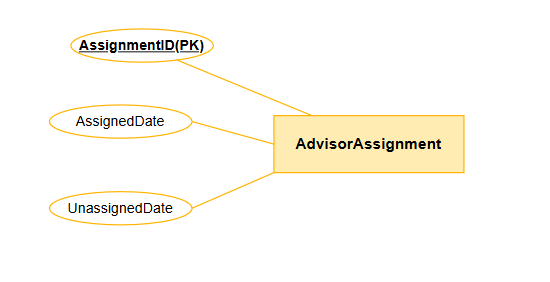
\includegraphics[width=0.8\textwidth]{advisorassignment.png}
    \caption{}
\end{figure}
\noindent
\begin{tabular}{p{0.55\textwidth}p{0.40\textwidth}}
\vspace{0pt}
This is the AdvisorAssignment entity, managing the many-to-many relationship between students and instructors with temporal validity. AdvisorAssignment has 5 attributes. AssignmentID is the auto-incremented primary key. StudentID (FK) references the student being advised. InstructorID (FK) references the assigned advisor (instructor). AssignedDate records when the advising relationship began (default: TODAY). UnassignedDate records when the relationship ended (NULL if currently active). A CHECK constraint ensures UnassignedDate is NULL or $>$ AssignedDate. IsActive is derived: UnassignedDate IS NULL = Active. This temporal design enables auditing of historical advisor relationships. Both FKs use ON DELETE NO ACTION to prevent accidental deletion of student/instructor records. The entity supports multiple advisors per student and multiple students per advisor across time.
&
\vspace{0pt}
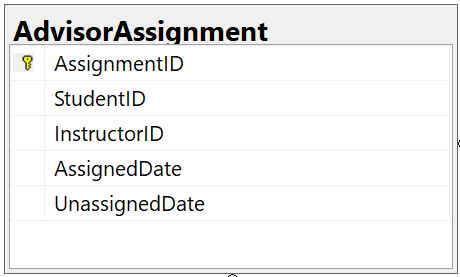
\includegraphics[width=0.95\linewidth]{advisorAssignment_tb.png}
\\
\end{tabular}

\vspace{1.5cm}


% ========================================================================================
% LOOKUP TABLES SECTION
% ========================================================================================

\section{LOOKUP TABLES}

Lookup tables contain reference data that doesn't change frequently and provides controlled vocabularies for the system.

% ========================================================================================
% SECTION 10: GOALCATEGORYLOOKUP
% ========================================================================================

\subsection{GOALCATEGORYLOOKUP}
\begin{figure}[H]
     \centering
    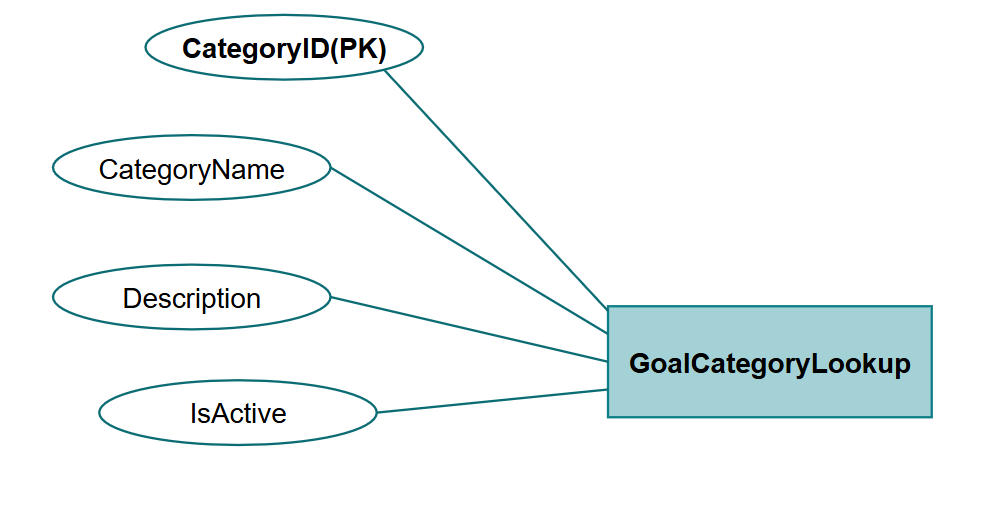
\includegraphics[width=0.8\textwidth]{goalcategorylookup.png}
    \caption{}
\end{figure}
\noindent
\begin{tabular}{p{0.55\textwidth}p{0.40\textwidth}}
\vspace{0pt}
GoalCategoryLookup is a master lookup table containing predefined goal categories for classification. It has 4 attributes: CategoryID (PK, IDENTITY), CategoryName (UNIQUE), Description, and IsActive. Standard values include: Academic (study/GPA goals), Skill Development (professional skills), Career (internships/employment), Personal (health/improvement), Project (assignments), and Certificate (professional certifications). This lookup enables consistent goal categorization across the system and prevents data anomalies from invalid category values. The UNIQUE constraint on CategoryName ensures no duplicate categories exist.
&
\vspace{0pt}
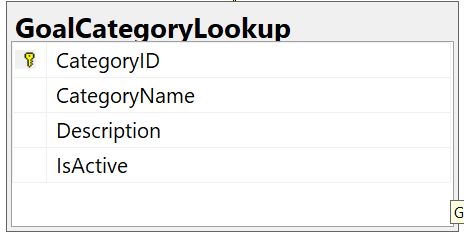
\includegraphics[width=0.95\linewidth]{goalcategorylookup_tb.png}
\\
\end{tabular}

\vspace{1cm}

% ========================================================================================
% SECTION 11: GOALSTATUSLOOKUP
% ========================================================================================

\subsection{GOALSTATUSLOOKUP}
\begin{figure}[H]
     \centering
    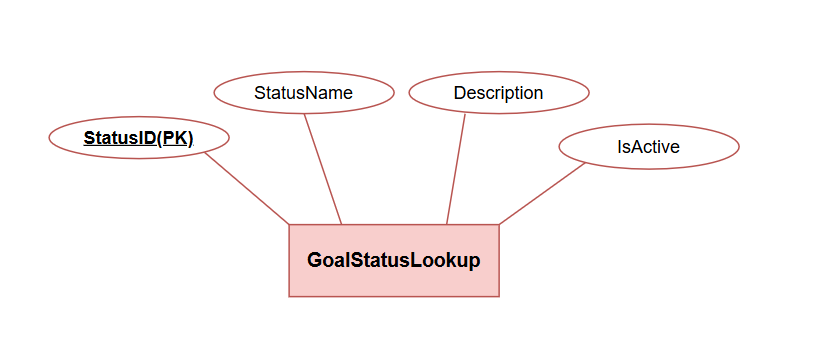
\includegraphics[width=0.8\textwidth]{goalstatuslookup.png}
    \caption{}
\end{figure}
\noindent
\begin{tabular}{p{0.55\textwidth}p{0.40\textwidth}}
\vspace{0pt}
GoalStatusLookup is a master lookup table containing goal state values. It has 4 attributes: StatusID (PK, IDENTITY), StatusName (UNIQUE, CHECK constraint), Description, and IsActive. Allowed status values are: Active (goal in progress), Completed (successfully achieved), Failed (not achieved), and Cancelled (explicitly terminated). The CHECK constraint restricts StatusName to these four values, enforcing data integrity at the database level. This prevents invalid goal statuses and ensures consistent state tracking throughout the system.
&
\vspace{0pt}
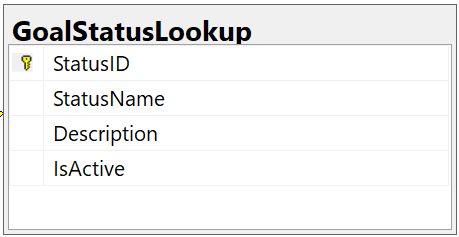
\includegraphics[width=0.95\linewidth]{goalstatuslookup_tb.png}
\\
\end{tabular}

\vspace{1cm}

% ========================================================================================
% SECTION 12: SEMESTERLOOKUP
% ========================================================================================

\subsection{SEMESTERLOOKUP}
\begin{figure}[H]
     \centering
    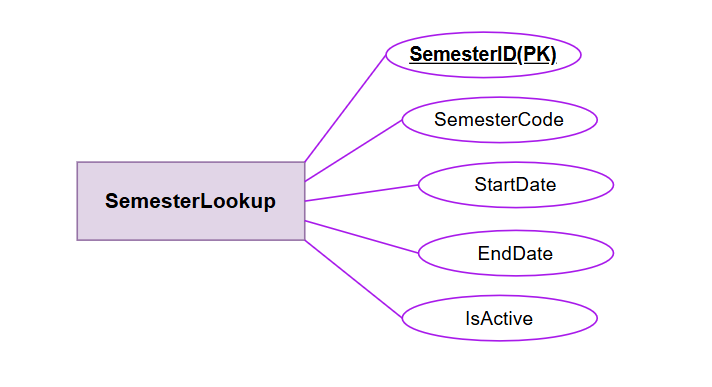
\includegraphics[width=0.5\textwidth]{semesterlookup.png}
    \caption{}
\end{figure}
\noindent
\begin{tabular}{p{0.55\textwidth}p{0.40\textwidth}}
\vspace{0pt}
SemesterLookup is a master lookup table containing academic semester reference data. It has 5 attributes: SemesterID (PK, IDENTITY), SemesterCode (UNIQUE), StartDate, EndDate, and IsActive. SemesterCode uses standardized format (e.g., ``Fall2024'', ``Spring2025''). A CHECK constraint ensures EndDate $>$ StartDate, preventing invalid date ranges. Example data includes: Fall2024 (09/01--12/31), Spring2025 (01/01--05/31), Summer2025 (06/01--08/31), Fall2025 (09/01--12/31). This lookup enables temporal organization of enrollments, goals, and progress tracking across academic periods.
&
\vspace{0pt}
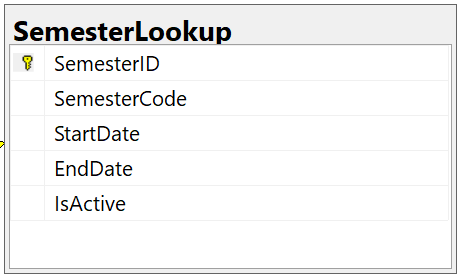
\includegraphics[width=0.95\linewidth]{semesterlookup_tb.png}
\\
\end{tabular}






\section{NORMAL FORM}

% Thảo luận về 3NF...
BEFORE (Violates 3NF):
   COURSE: CourseID → CourseName, Credits, InstructorID, InstructorName
   Transitive: CourseID → InstructorID → InstructorName \\
   \begin{figure}[H]
     \centering
    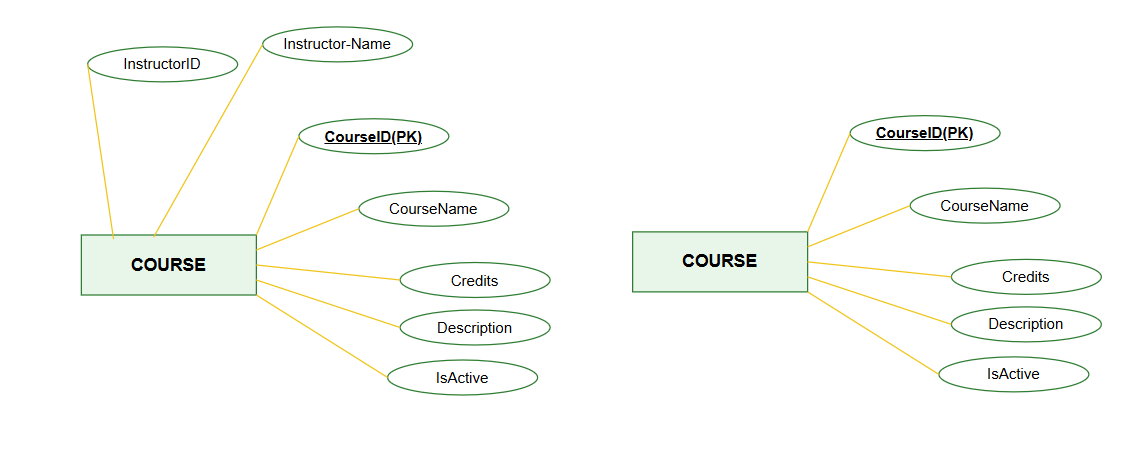
\includegraphics[width=0.8\textwidth]{NF.png}
    \caption{}
\end{figure}
 AFTER (3NF):
   COURSE: CourseID → CourseName, Credits
   ENROLLMENT: StudentID, CourseID, SemesterID → InstructorID
   No transitive dependencies 
   
\section{FULL DIAGRAM}
\begin{figure}[H]
   \centering
   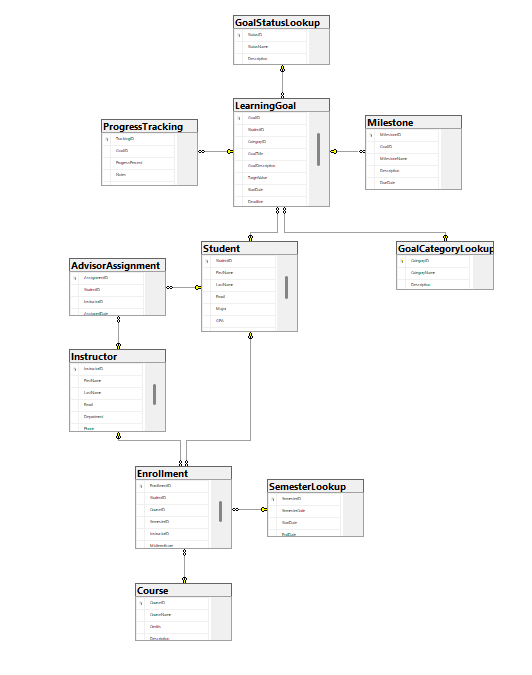
\includegraphics[width=0.9\textwidth]{fulldiagram.png}
   \caption{Full Diagram}
 \end{figure}








% ================================
% CHƯƠNG V: SQL COMMAND
% ================================

\chapter{SQL COMMAND}

% ============================================================
\section{Query Using ORDER BY}
% ============================================================

\textbf{Topic:} Sorting students by academic performance

\begin{lstlisting}[language=SQL, caption=ORDER BY Example]
SELECT
    StudentID,
    FirstName + ' ' + LastName AS FullName,
    Major,
    GPA
FROM Student
ORDER BY GPA DESC, StudentID ASC;
\end{lstlisting}
\textbf{Purpose of the query:} The Academic Affairs Office needs a comprehensive list of all students in the school, prioritizing those with the highest academic achievements. This list will be used to prepare for scholarship distribution and recognition ceremonies. Students must be sorted in descending order by GPA (highest to lowest), with StudentID as the secondary sort key in ascending order.\\
\textbf{Result:}
\begin{figure}[H]
     \centering
    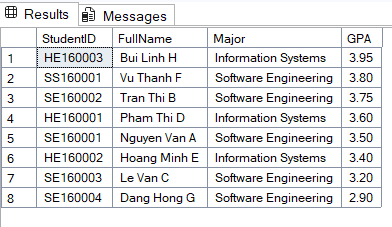
\includegraphics[width=0.6\textwidth]{Ques1.png}
    \caption{}
\end{figure}
\vspace{0cm}

% ============================================================
\section{Query Using INNER JOIN}
% ============================================================

\textbf{Topic:} Retrieving detailed student transcript

\begin{lstlisting}[language=SQL, caption=INNER JOIN Example]
SELECT
    s.FirstName,
    s.LastName,
    c.CourseName,
    e.MidtermScore,
    e.FinalScore
FROM
    Student s
INNER JOIN
    Enrollment e ON s.StudentID = e.StudentID
INNER JOIN
    Course c ON e.CourseID = c.CourseID
WHERE
    s.StudentID = 'SE160002';
\end{lstlisting}

\textbf{Purpose of the query:} Student 'SE160002' wants to view his/her complete transcript. This query joins three tables (Student, Enrollment, and Course) to display the student's first name, last name, course names, midterm scores, and final scores for all courses the student has enrolled in.\\
\textbf{Result:}
\begin{figure}[H]
     \centering
    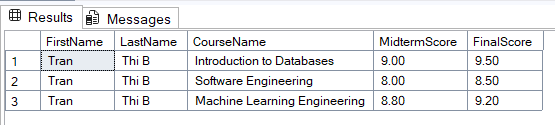
\includegraphics[width=0.8\textwidth]{Ques2.png}
    \caption{}
\end{figure}
\vspace{0cm}

% ============================================================
\section{Query Using AGGREGATE FUNCTIONS}
% ============================================================

\textbf{Topic:} School KPI (Key Performance Indicators) statistics

\begin{lstlisting}[language=SQL, caption=AGGREGATE FUNCTIONS Example]
SELECT
    (SELECT COUNT(*)
     FROM Student
     WHERE IsActive = 1) AS TotalActiveStudents,
    (SELECT AVG(CAST(GPA AS DECIMAL(5,2))) FROM Student) AS AverageGPA,
    (SELECT COUNT(*)
     FROM LearningGoal lg
     JOIN GoalStatusLookup gs ON gs.StatusID = lg.StatusID
     WHERE gs.StatusName = 'Active') AS TotalActiveGoals;
\end{lstlisting}

\textbf{Purpose of the query:} The school dashboard needs to display three key performance indicators (KPI):
\begin{itemize}
    \item \textit{TotalActiveStudents:} Count of all active students (IsActive = 1)
    \item \textit{AverageGPA:} Average GPA of all students
    \item \textit{TotalActiveGoals:} Total count of learning goals currently in 'Active' status
\end{itemize}
This single query returns all three metrics using correlated subqueries with aggregate functions.
\textbf{Result:}
\begin{figure}[H]
     \centering
    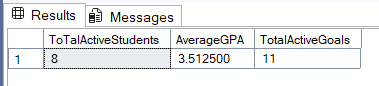
\includegraphics[width=0.8\textwidth]{Ques3.png}
    \caption{}
\end{figure}
\vspace{0cm}

% ============================================================
\section{Query Using GROUP BY and HAVING Clauses}
% ============================================================

\textbf{Topic:} Instructor performance evaluation

\begin{lstlisting}[language=SQL, caption=GROUP BY and HAVING Example]
SELECT
    e.InstructorID,
    AVG(e.FinalScore) AS AvgFinalScore,
    COUNT(*) AS NumEnrollments
FROM Enrollment e
GROUP BY e.InstructorID
HAVING AVG(e.FinalScore) > 8.5
    AND COUNT(*) >= 2
ORDER BY AvgFinalScore DESC;
\end{lstlisting}

\textbf{Purpose of the query:} The department wants to identify instructors with strong teaching performance based on student grades. This query groups enrollment records by instructor and filters to show only instructors whose average final score exceeds 8.5 AND have taught at least 2 courses. Results are sorted by average score in descending order to highlight top performers.
\textbf{Result:}
\begin{figure}[H]
     \centering
    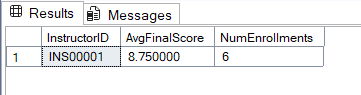
\includegraphics[width=0.6\textwidth]{ques4.png}
    \caption{}
\end{figure}
\vspace{0.5cm}

% ============================================================
\section{Query Using a Sub-query as a Relation}
% ============================================================

\textbf{Topic:} Finding outstanding students (compared to major average)

\begin{lstlisting}[language=SQL, caption=Sub-query as Relation Example]
SELECT
    s.StudentID,
    s.FirstName + ' ' + s.LastName AS FullName,
    s.Major,
    s.GPA
FROM Student s
INNER JOIN (
    SELECT Major, AVG(GPA) AS AvgMajorGPA
    FROM Student
    GROUP BY Major
) mg ON s.Major = mg.Major
WHERE s.GPA > mg.AvgMajorGPA
ORDER BY s.Major, s.GPA DESC;
\end{lstlisting}

\textbf{Purpose of the query:} Identify high-achieving students whose GPA is higher than the average GPA of their major program. This query uses a derived table (subquery in FROM clause) to calculate the average GPA for each major, then joins it with the Student table to compare individual students against their major's average. Only students exceeding their major's average GPA are displayed.
\textbf{Result:}
\begin{figure}[H]
     \centering
    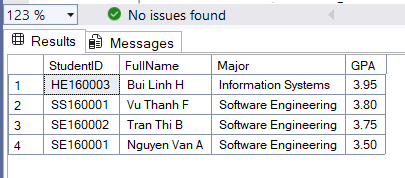
\includegraphics[width=0.6\textwidth]{ques5.png}
    \caption{}
\end{figure}
\vspace{0cm}

% ============================================================
\section{Query Using Partial Matching in WHERE Clause}
% ============================================================

\textbf{Topic:} Building a learning goal search feature

\begin{lstlisting}[language=SQL, caption=Partial Matching Example]
SELECT
    GoalID,
    GoalTitle
FROM
    LearningGoal
WHERE
    (GoalTitle LIKE N'%Docker%' OR GoalTitle LIKE N'%Kubernetes%')
    OR
    (GoalDescription LIKE N'%Docker%' OR GoalDescription LIKE N'%Kubernetes%');
\end{lstlisting}

\textbf{Purpose of the query:} Users (students or advisors) need to search for learning goals related to DevOps skill development. This query returns GoalID and GoalTitle of all goals where either the GoalTitle or GoalDescription contains the keywords 'Docker' OR 'Kubernetes'. The LIKE operator with wildcard (\%) enables flexible partial string matching across multiple columns.
\textbf{Result:}
\begin{figure}[H]
     \centering
    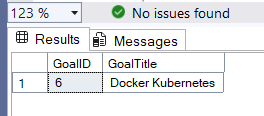
\includegraphics[width=0.6\textwidth]{ques6.png}
    \caption{}
\end{figure}
\vspace{0.5cm}

% ============================================================
\section{Query Using a Self-Join}
% ============================================================

\textbf{Topic:} Finding pairs of students in the same class

\begin{lstlisting}[language=SQL, caption=Self-Join Example]
SELECT
    e1.CourseID,
    e1.StudentID AS Student1_ID,
    e2.StudentID AS Student2_ID
FROM
    Enrollment e1
INNER JOIN
    Enrollment e2 ON e1.CourseID = e2.CourseID
    AND e1.SemesterID = e2.SemesterID
WHERE
    e1.StudentID < e2.StudentID;
\end{lstlisting}

\textbf{Purpose of the query:} Identify pairs of students who have enrolled in the same course (CourseID) during the same semester (SemesterID). This query uses a self-join on the Enrollment table with two aliases (e1 and e2). Critical considerations:
\begin{itemize}
    \item The WHERE clause ensures a student is never paired with themselves (e1.StudentID < e2.StudentID)
    \item Each pair appears only once (avoids showing both (SE160001, SE160002) and (SE160002, SE160001))
    \item Results display CourseID, Student1\_ID, and Student2\_ID
\end{itemize}
\textbf{Result:}
\begin{figure}[H]
     \centering
    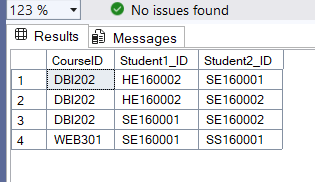
\includegraphics[width=0.8\textwidth]{ques7.png}
    \caption{}
\end{figure}
\vspace{0.5cm}
\clearpage
% ============================================================
\section{Stored Procedure}
% ============================================================

\textbf{Topic:} Creating a stored procedure to add a new course

\begin{lstlisting}[language=SQL, caption=Stored Procedure Example]
CREATE PROCEDURE sp_AddNewCourse
    @CourseID VARCHAR(10),
    @CourseName NVARCHAR(200),
    @Credits INT
AS
BEGIN
    SET NOCOUNT ON;
    BEGIN TRY
        INSERT INTO Course (CourseID, CourseName, Credits)
        VALUES (@CourseID, @CourseName, @Credits);
 
        PRINT 'New course has been added successfully.';
        SELECT *
        FROM Course
    END TRY
    BEGIN CATCH
        PRINT 'Error: ' + ERROR_MESSAGE();
        RAISERROR('Unable to add course. An error has occurred.', 16, 1);
    END CATCH
END;
-- Example execution:
EXEC sp_AddNewCourse @CourseID = 'NEW101', @CourseName = N'New Course Title', @Credits = 3;
\end{lstlisting}

\textbf{Purpose of the query:} This procedure automates the process of adding a new course to the Course table. It accepts three input parameters (CourseID, CourseName, Credits) and inserts them into the database. Key points:
\begin{itemize}
    \item Fields not provided (Description, IsActive) will use their table defaults
    \item Includes basic error handling with TRY-CATCH block
    \item Uses SET NOCOUNT ON to suppress system messages
    \item Provides success and error messages
    \item Show all information of Course in database
\end{itemize}
\textbf{Result:}
\begin{figure}[H]
     \centering
    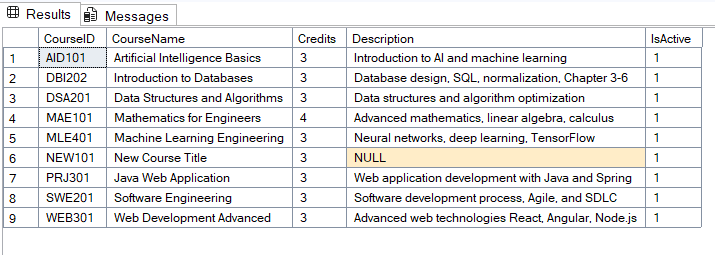
\includegraphics[width=0.8\textwidth]{ques8.png}
    \caption{}
\end{figure}
\vspace{0.5cm}

% ============================================================
\section{Trigger (Audit Logging)}
% ============================================================

\textbf{Topic:} Creating a trigger for student insertion audit logging

\begin{lstlisting}[language=SQL, caption=Trigger Example]
CREATE TRIGGER trg_AuditNewStudent
ON Student                    
AFTER INSERT                  
AS
BEGIN
    SET NOCOUNT ON;
 
   
    INSERT INTO AuditLog (
        TableName,
        Operation,
        RecordID,
        NewValue,
        ModifiedBy
    )
 
    
    SELECT
        'Student',                              
        'INSERT',                               
        i.StudentID,                            
        i.FirstName + ' ' + i.LastName,         
        'SYSTEM'                               
    FROM
        inserted i; 
END                 
\end{lstlisting}

\textbf{Purpose of the query:} This trigger automatically creates an audit log entry whenever a new student is added to the system. It captures:
\begin{itemize}
    \item \textit{TableName:} 'Student'
    \item \textit{Operation:} 'INSERT'
    \item \textit{RecordID:} The new StudentID
    \item \textit{NewValue:} Student's full name (FirstName + LastName concatenation)
    \item \textit{ModifiedBy:} 'SYSTEM' (indicating automatic enrollment action)
\end{itemize}
The trigger uses the special 'inserted' table to access values of newly added records, ensuring audit compliance and data tracking for system transparency.\\
\vfill

\begin{center}
    {\fontsize{50pt}{0}\selectfont \textbf{THE END}}
\end{center}

\vfill
% ================================
% KẾT THÚC TÀI LIỆU
% ================================

\end{document}